\documentclass[runningheads]{llncs}

\usepackage{iftex}
\ifPDFTeX
  \usepackage[T2A]{fontenc}
  \usepackage[utf8]{inputenc}
  \usepackage[russian,english]{babel}
\else
  \usepackage{fontspec}
  \setmainfont{Times New Roman}
  \setsansfont{Arial}
  \setmonofont{Arial Unicode MS}
  \usepackage{polyglossia}
  \setmainlanguage{russian}
  \setotherlanguage{english}
  \newfontfamily\cyrillicfont{Times New Roman}[Script=Cyrillic]
  \newfontfamily\cyrillicfontsf{Arial}[Script=Cyrillic]
  \newfontfamily\cyrillicfonttt{Arial Unicode MS}
\fi
\usepackage{amsmath}
\usepackage{amssymb}
\usepackage{booktabs}
\usepackage{graphicx}
\usepackage{array}
\usepackage{url}

\ifPDFTeX
  \selectlanguage{russian}
\fi

\begin{document}
\emergencystretch=3em

\title{RAG-LLM-параметризация формальных моделей координации в складской многоагентной робототехнической системе}
\titlerunning{RAG-LLM-параметризация координации MAS}

\author{Анонимизировано для рецензирования}
\authorrunning{Анонимизировано}
\institute{Анонимизировано для рецензирования}

\maketitle

\begin{abstract}
Объектом исследования является складская многоагентная робототехническая система, в которой группа мобильных роботов выполняет транспортные заявки при наличии общих коридоров, ограниченной вместимости зон погрузки и локальных рисков столкновения. Предмет исследования -- механизм многоуровневого принятия решений, связывающий текстовые правила эксплуатации склада с формальными моделями распределения задач и выбора маршрутов. Рассматриваемая проблема состоит в том, что классические модели Contract Net и игр с заторами дают воспроизводимые решения, но требуют заранее заданных численных параметров, тогда как часть эксплуатационного контекста формулируется в текстовом виде: инспекционный трафик, временные ограничения зон, приоритеты движения и правила дозированного выпуска роботов. Предложен подход RAG-LLM-параметризации: локальная языковая модель Ollama, получающая правила из векторной базы SQLite через RAG, формирует не действия роботов, а проверяемый вектор стратегии: веса целевой функции, списки допуска и ожидания агентов, ограничения на активные задания и штрафы перегруженных ребер. Далее этот вектор используется формальными уровнями: Contract Net назначает заявки, конечная игра с заторами выбирает маршруты, а индивидуальные контроллеры Webots выполняют локальное движение с A* и предотвращением столкновений. Новизна работы заключается в явном разделении языкового, тактического и операционного уровней, а также в логико-алгебраической модели, где LLM рассматривается как ограниченный параметризатор формальных процедур, а не как управляющий контур. Эксперименты показывают, что эффект подхода проявляется не в малых сценах, а в конфликтной конфигурации с 8 роботами и 9 заявками: makespan уменьшается с 294.0 до 252.0 с, а суммарное ожидание -- с 472.5 до 28.5 с при росте длины маршрутов за счет обходов.

\keywords{многоагентные системы \and складская робототехника \and Contract Net Protocol \and игры с заторами \and RAG \and локальные языковые модели \and Webots}
\end{abstract}

\section{Введение}

Складская робототехническая система с несколькими мобильными роботами является характерным примером многоагентной системы, в которой производительность определяется не только локальной скоростью движения, но и согласованностью решений на разных уровнях. Роботы конкурируют за транспортные заявки, используют общие коридоры, ожидают освобождения зон погрузки и разгрузки, а также должны предотвращать столкновения на уровне локального движения. Поэтому простая централизованная диспетчеризация быстро становится недостаточной: она либо игнорирует локальные конфликты, либо превращается в трудно объяснимый монолитный контроллер.

Классические формальные модели хорошо решают отдельные части этой задачи. Протокол Contract Net естественно описывает распределение заявок между агентами, игры с заторами -- выбор маршрутов в общей транспортной инфраструктуре, а локальные планировщики движения -- обход препятствий. Однако на практике параметры этих моделей не всегда задаются числовыми таблицами. Часть правил эксплуатации склада имеет текстовую форму: центральный коридор временно используется инспекционной тележкой, в зоне погрузки одновременно должен находиться только один робот, при равенстве приоритетов действует правостороннее движение, а выпуск роботов следует дозировать, чтобы не создавать пробку. Такое правило должно быть переведено в веса, ограничения и допустимые множества агентов, прежде чем формальные модели смогут его использовать.

Объектом исследования в данной работе является складская многоагентная робототехническая система, выполняющая поток транспортных заявок. Предмет исследования -- механизм многоуровневого принятия решений, в котором текстовые правила склада преобразуются в параметры формальных моделей назначения задач, выбора маршрутов и локального движения. Исследовательская проблема формулируется следующим образом: как включить LLM в многоагентную робототехническую систему так, чтобы использовать ее способность интерпретировать текстовые правила, но не потерять проверяемость, воспроизводимость и безопасность формальных алгоритмов.

Гипотеза исследования: LLM полезна не как генератор действий роботов, а как стратегический параметризатор. Если ограничить выход LLM типизированным вектором стратегии и пропустить его через guardrails, то дальнейшие решения могут оставаться формальными: Contract Net распределяет задачи, игра с заторами выбирает маршруты, а индивидуальные контроллеры обеспечивают движение и предотвращение столкновений. В такой архитектуре выигрыш должен проявляться не в малых сценах, где формальных правил достаточно, а в конфликтных конфигурациях с несколькими альтернативными маршрутами и текстовым контекстом, отсутствующим в простом fallback.

Цель работы состоит в разработке и экспериментальной оценке такого многоуровневого подхода. Для достижения цели решаются четыре задачи: формализовать складскую транспортную задачу как логико-алгебраическую модель; определить поток данных между RAG-LLM, Contract Net, игрой с заторами и локальными контроллерами; реализовать систему в Webots с индивидуальными контроллерами роботов и сетевым координатором; оценить, при каких размерах сцены и конфигурациях маршрутов LLM дает измеримый эффект.

Научная новизна работы заключается в модели RAG-LLM-параметризации формальных многоагентных процедур. В отличие от подходов, где языковая модель генерирует программы или команды роботу, здесь LLM не имеет доступа к колесным скоростям и траекториям. Она формирует только проверяемый стратегический вектор: веса дедлайна, пути, батареи и заторов, списки $A^{go}$ и $A^{hold}$, ограничения на число активных назначений и мягкие запреты ребер. Практический эффект состоит в снижении ожидания и makespan в сценариях, где текстовое правило о перегрузке центрального коридора должно изменить распределение потоков по обходным маршрутам.

\section{Обзор литературы}

Исследование опирается на три группы работ. Первая группа посвящена распределению задач в многоагентных робототехнических системах. Вторая описывает теоретико-игровую маршрутизацию в общих сетях. Третья связана с использованием языковых моделей в робототехнике.

Первая группа относится к Multi-Robot Task Allocation (MRTA). Работа Gerkey и Matari{\'c}~\cite{GerkeyMataric2004MRTA} задала таксономию MRTA и связала распределение задач между роботами с задачами оптимизации. Для складской транспортной системы важен случай, где каждая заявка назначается одному роботу, а робот одновременно выполняет не более одной заявки. Протокол Contract Net~\cite{Smith1980ContractNet} предлагает для такой ситуации распределенный механизм заявок и ставок: агент оценивает задачу локально, а координатор выбирает победителя. Обзоры и развитие рыночных подходов~\cite{Dias2006MarketSurvey,ZlotStentz2006ComplexTasks} показывают, что аукционные механизмы хорошо масштабируются и допускают децентрализованную интерпретацию полезности, но качество результата критически зависит от состава функции ставки. Для складских транспортных систем это согласуется с обзорами AGV/AMR-управления~\cite{LeAnhDeKoster2006AGV,Fragapane2021AMR}, где подчеркивается зависимость эффективности от диспетчерских правил, планирования движения и структуры транспортной сети. Следовательно, нерешенным остается вопрос, как адаптировать веса и ограничения функции ставки при изменении эксплуатационного контекста склада.

Вторая группа работ описывает выбор маршрутов в общей инфраструктуре. Игры с заторами, введенные Rosenthal~\cite{Rosenthal1973Congestion}, моделируют ситуацию, когда стоимость ресурса растет с числом пользователей. Monderer и Shapley~\cite{MondererShapley1996Potential} связали такие модели с потенциальными играми, а Roughgarden и Tardos~\cite{RoughgardenTardos2002SelfishRouting} показали, что эгоистичный выбор маршрутов может быть неэффективным. Для склада эти результаты означают, что общий коридор может рассматриваться как ресурс с возрастающей стоимостью. На операционном уровне такой выбор связан с классическими задачами планирования движения~\cite{LaValle2006Planning}, поиска пути и предотвращения столкновений: A*~\cite{Hart1968AStar}, потенциальные поля~\cite{Khatib1986PotentialFields}, Dynamic Window Approach~\cite{Fox1997DWA}, а также методы Multi-Agent Path Finding~\cite{YuLaValle2013MAPF,Sharon2015CBS} задают алгоритмическую основу для маршрутизации и локального движения. Однако сама величина штрафа за перегрузку зависит от контекста: нормальный режим, инспекция центрального прохода, временное обслуживание стеллажей или повышенный приоритет разгрузки. Поэтому в данной работе MAPF не заменяет игру с заторами, а используется как близкая формальная рамка, показывающая, что конфликтность маршрутов должна учитываться явно.

Третья группа связана с LLM и RAG. Подход Retrieval-Augmented Generation~\cite{Lewis2020RAG} позволяет передавать языковой модели релевантные документы из внешнего хранилища, уменьшая зависимость от параметрической памяти. Методы chain-of-thought и ReAct~\cite{Wei2022CoT,Yao2023ReAct} показали, что языковые модели могут использовать промежуточные рассуждения и связывать их с действиями, а современные обзоры агентных LLM-систем~\cite{Xi2023LLMAgentSurvey} фиксируют переход от разовых ответов к циклам планирования, памяти и инструментального взаимодействия. В робототехнике SayCan~\cite{Ahn2022SayCan}, Code as Policies~\cite{Liang2022CodeAsPolicies} и PaLM-E~\cite{Driess2023PalmE} демонстрируют, что языковые модели могут связывать инструкции с действиями, программами или мультимодальным состоянием. Вместе с тем эти подходы поднимают проблему безопасности: прямой вывод LLM не должен без проверки попадать в контур управления физическим агентом.

Таким образом, в литературе существуют проверяемые модели назначения и маршрутизации, а также методы интерпретации текстового контекста с помощью LLM. Недостаточно разработан механизм их соединения, при котором LLM не заменяет формальные алгоритмы, а задает им ограниченный и проверяемый набор параметров. Именно этот разрыв определяет место предлагаемого подхода: RAG-LLM используется для преобразования текстовых правил склада в стратегический вектор, а все решения с физическим смыслом остаются за формальными моделями и локальными контроллерами.

Сравнительное позиционирование предлагаемой работы приведено в табл.~\ref{tab:related-position}. Таблица показывает, что отдельные исследовательские линии решают важные частные задачи, но не задают полного контура, в котором текстовые правила эксплуатации склада влияют на формальные модели, сохраняя проверяемость результата. Для рассматриваемой системы принципиально, что языковая модель не конкурирует с алгоритмами MRTA, MAPF или локального управления. Она используется на другом уровне абстракции: преобразует неструктурированный контекст в параметры уже заданных моделей.

\begin{table}[!htbp]
\centering
\caption{Позиционирование предлагаемого подхода относительно смежных работ.}
\label{tab:related-position}
\scriptsize
\begin{tabular}{p{0.2\textwidth}p{0.25\textwidth}p{0.25\textwidth}p{0.22\textwidth}}
\toprule
Направление & Что решает & Ограничение для данной задачи & Использование в работе \\
\midrule
MRTA и Contract Net & Распределение задач между роботами по ставкам и полезности & Требует заданной функции ставки и правил допуска & Тактическое назначение заявок \\
Игры с заторами & Учет роста стоимости общих ресурсов при конкуренции агентов & Не интерпретируют текстовый контекст склада & Выбор маршрутов и штраф перегруженных ребер \\
MAPF и локальное движение & Конфликты траекторий, поиск пути, объезд препятствий & Слабо описывают эксплуатационные правила высокого уровня & Операционное исполнение и безопасность \\
RAG и LLM-агенты & Извлечение и интерпретация текстовых правил & Нужны ограничения на выход и запрет прямого управления & Стратегическая параметризация формальных моделей \\
Складские AGV/AMR-системы & Диспетчеризация, маршрутизация и управление транспортным потоком & Часто разделяют правила эксплуатации и модель принятия решений & Интегральный сценарий Webots и вычислительный эксперимент \\
\bottomrule
\end{tabular}
\end{table}

\section{Предлагаемый подход}

Ключевая идея подхода состоит в разделении принятия решений на три уровня. Стратегический уровень отвечает за интерпретацию эксплуатационного контекста: какие правила актуальны, насколько опасен центральный коридор, сколько роботов следует выпускать одновременно и какие агенты должны подождать. Тактический уровень превращает стратегию в назначения и маршруты: Contract Net распределяет заявки между агентами, а игра с заторами выбирает профиль маршрутов. Операционный уровень выполняет выбранный маршрут в Webots: индивидуальный контроллер робота строит локальный путь, объезжает препятствия и сообщает события о погрузке, разгрузке или необходимости перепланирования.

Принципиально важно, что LLM не является источником траекторий. Ее выход имеет фиксированную структуру и проходит проверку. Поэтому ошибка или недоступность LLM не разрушает систему: вместо нее используется fallback-стратегия, а тактический и операционный уровни продолжают работать без изменения.

\begin{figure}[!htbp]
\centering
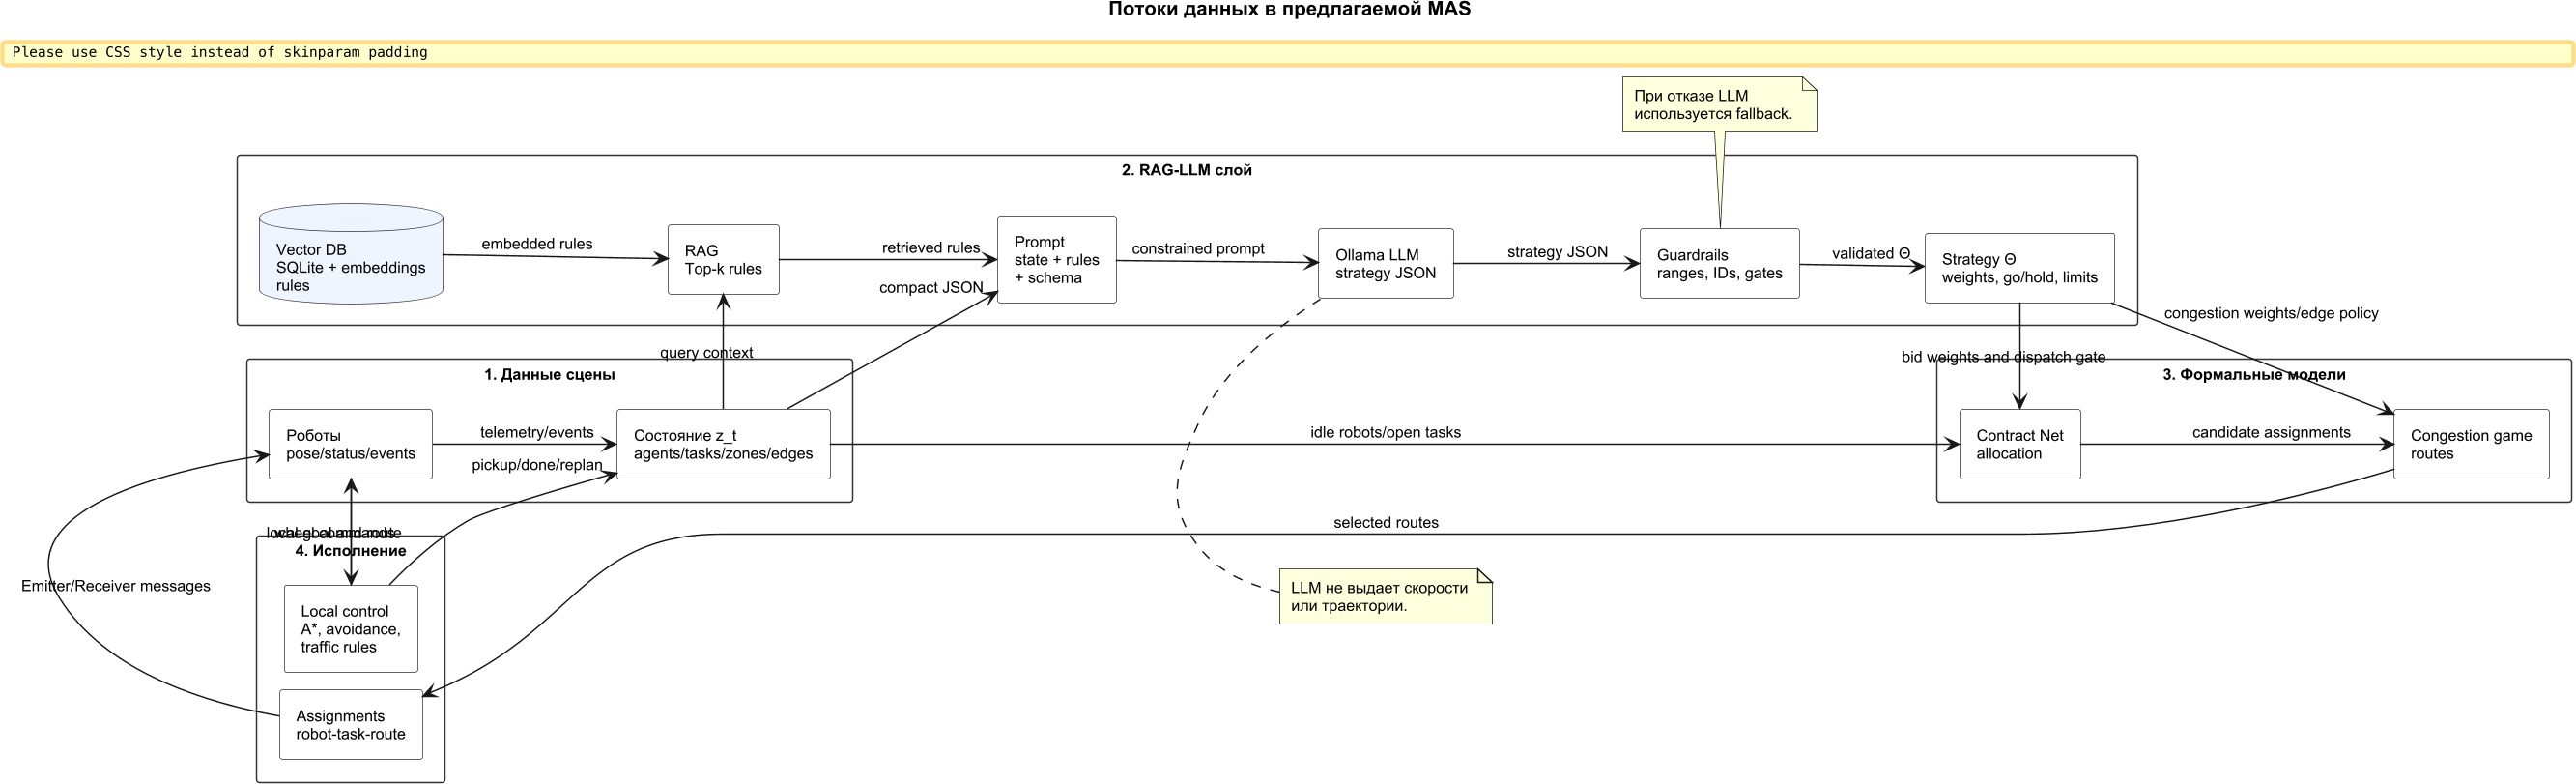
\includegraphics[width=0.96\textwidth]{figures/uml/article_data_flow.png}
\caption{Диаграмма потоков данных предлагаемого подхода: текстовые правила и состояние склада преобразуются в стратегический вектор, после чего формальные модели выполняют назначение задач и выбор маршрутов.}
\label{fig:data-flow}
\end{figure}

Диаграмма потоков данных на рис.~\ref{fig:data-flow} задает основную логику системы. Роботы передают координаты, статусы задач и события локальных конфликтов. Из этих сообщений формируется состояние $z_t$, содержащее открытые заявки, свободных агентов, занятость зон и текущую нагрузку ребер. Это состояние используется двумя путями. Во-первых, оно напрямую поступает в Contract Net и игру с заторами. Во-вторых, оно является запросом к векторной базе правил, где хранятся документы о координатной системе склада, правиле правой стороны, политике перегрузки, динамическом предотвращении столкновений и диспетчерском дозировании.

RAG-подсистема возвращает набор релевантных правил, которые вместе с $z_t$ и JSON-схемой образуют prompt для локальной Ollama-модели. Ответ LLM имеет вид стратегического JSON, но до использования проходит guardrails: проверяются типы, диапазоны весов, допустимость идентификаторов роботов и ребер, а также ограничивается число новых назначений. Результатом является стратегический вектор, который параметризует формальные модели, но не отменяет их.

Векторная база в реализации является локальной SQLite-БД, в которой каждый документ хранится как кортеж
\[
d_i=(id_i, text_i, tags_i, v_i),
\]
где $id_i$ -- идентификатор правила, $text_i$ -- текст правила, $tags_i$ -- тематические метки, $v_i \in \mathbb{R}^k$ -- векторное представление. Векторизация выполнена локально на PyTorch: текст правила преобразуется в мешок нормализованных токенов, после чего строится плотный вектор по фиксированному словарю признаков. Такой вариант не претендует на качество специализированных embedding-моделей, но обеспечивает воспроизводимость без внешних API и демонстрирует сам принцип RAG-контура. Запрос $q(z_t)$ формируется из компактного состояния склада: числа свободных роботов, активных задач, занятости зон, наиболее загруженных ребер и признаков локальных конфликтов. Результатом поиска является упорядоченное множество
\[
Q(z_t)=\{d_{i_1},\ldots,d_{i_k}\},
\]
отобранное по косинусной близости между вектором запроса и векторами правил.

Содержательно в базе выделены пять типов правил. Первый тип фиксирует координатную систему и ориентацию склада, чтобы исключить неоднозначность ``верх--низ'' и ``лево--право'' при описании pickup/dropoff-зон. Второй тип задает правила движения: правосторонний приоритет, уступание на перекрестках и запрет одновременного входа в узкое место. Третий тип описывает политику заторов: при высокой нагрузке центрального коридора предпочтительны обходные маршруты, даже если их геометрическая длина больше. Четвертый тип задает ограничения зон: повторные задания одной семьи не должны одновременно занимать одну pickup/dropoff-пару. Пятый тип описывает отказоустойчивость: при тайм-ауте Ollama применяется fallback, сохраняющий тот же формальный pipeline.

\begin{table}[!htbp]
\centering
\caption{Входы и выходы RAG-LLM-контура.}
\label{tab:rag-io}
\scriptsize
\begin{tabular}{p{0.18\textwidth}p{0.34\textwidth}p{0.38\textwidth}}
\toprule
Компонент & Вход & Выход \\
\midrule
Vector DB & Текстовые правила склада, теги, PyTorch-векторы & Top-$k$ релевантных правил и их идентификаторы \\
RAG retriever & Компактное состояние $z_t$ и вектор запроса $q(z_t)$ & Список документов для prompt и журнал сходства \\
Prompt builder & $z_t$, найденные правила, JSON-схема ответа & Ограниченный prompt без инструкций прямого управления \\
Ollama LLM & Prompt со схемой и правилами & JSON-кандидат стратегии: веса, лимиты, go/hold, edge policy \\
Guardrails & JSON-кандидат, допустимые множества агентов и ребер & Валидный стратегический вектор $\Theta$ или fallback \\
\bottomrule
\end{tabular}
\end{table}

\begin{table}[!htbp]
\centering
\caption{Распределение ответственности между уровнями принятия решений.}
\label{tab:levels}
\scriptsize
\begin{tabular}{p{0.2\textwidth}p{0.27\textwidth}p{0.27\textwidth}p{0.18\textwidth}}
\toprule
Уровень & Входные данные & Выходные данные & Метод \\
\midrule
Стратегический & $z_t$, правила из vector DB, JSON-схема & Стратегия: веса, $A^{go}$, $A^{hold}$, лимиты и штрафы ребер & RAG + Ollama + guardrails \\
Тактический & Стратегия, открытые заявки, свободные агенты, маршруты & Назначения агент--задача и профиль маршрутов & Contract Net, congestion game \\
Операционный & Назначение, маршрут, локальные препятствия & Скорости колес, события pickup/done/replan & A*, правила движения, локальный объезд \\
\bottomrule
\end{tabular}
\end{table}

Именно это разделение определяет заявленную новизну: LLM используется не как универсальный планировщик, а как адаптивный интерфейс между текстовыми правилами и формальными моделями. Поэтому эффект подхода должен измеряться не качеством языкового ответа как такового, а изменением метрик системы: времени завершения всех заявок, суммарного ожидания, числа обходных маршрутов и устойчивости при отказе LLM.

\section{Постановка задачи и логико-алгебраическая модель}

Формальная постановка нужна для того, чтобы отделить интерпретацию правил от исполнимых решений. Текстовые правила склада не входят в модель напрямую; они преобразуются в стратегический вектор. После этого все назначения, маршруты и локальные действия вычисляются над конечными множествами агентов, задач, ребер и допустимых маршрутов.

Пусть задано множество роботов
\[
A=\{a_1,\ldots,a_m\},
\]
множество транспортных заявок
\[
T=\{\tau_1,\ldots,\tau_n\},
\]
множество ребер складского графа
\[
E=\{e_1,\ldots,e_q\}
\]
и семейство допустимых маршрутов $R_\tau$ для каждой заявки $\tau \in T$. Заявка описывается кортежем
\[
\tau=(p_\tau,d_\tau,\rho_\tau,\delta_\tau,s_\tau),
\]
где $p_\tau$ и $d_\tau$ являются координатами погрузки и разгрузки, $\rho_\tau$ -- награда, $\delta_\tau$ -- дедлайн, $s_\tau \in \{\text{open},\text{assigned},\text{picked},\text{completed}\}$ -- статус. Робот описывается кортежем
\[
a=(x_a,\beta_a,\sigma_a,\tau_a),
\]
где $x_a$ -- положение, $\beta_a \in [0,1]$ -- заряд, $\sigma_a$ -- сетевой статус, $\tau_a$ -- текущая заявка или пустое значение.

Логико-алгебраическая структура задачи задается как
\[
\mathcal{M}=\langle A,T,E,R,P,F,C,U,\Pi\rangle,
\]
где $P$ -- множество предикатов состояния, $F$ -- множество функций оценки, $C$ -- множество ограничений, $U$ -- функции полезности, $\Pi$ -- множество политик управления. Используются следующие предикаты:
\[
\operatorname{Idle}(a),\quad \operatorname{Open}(\tau),\quad \operatorname{Feasible}(a,\tau,r),\quad \operatorname{Safe}(x_a,x_b),\quad \operatorname{Free}(e).
\]
Ограничения назначения имеют вид
\[
\sum_{\tau \in T} y_{a\tau} \le 1,\quad
\sum_{a \in A} y_{a\tau} \le 1,\quad
y_{a\tau}\in\{0,1\},
\]
где $y_{a\tau}=1$ означает, что робот $a$ назначен на заявку $\tau$. Для предотвращения перегрузки зон вводится отображение семейства задач $\phi:T\rightarrow \{A,B,C,\ldots\}$ и ограничение
\[
\sum_{\tau:\phi(\tau)=g} \mathbb{I}(s_\tau \notin \{\text{open},\text{completed}\}) \le 1.
\]
Оно означает, что повторные заявки одной pickup/dropoff-семьи не должны одновременно занимать одну и ту же зону.

Ставка робота в Contract Net определяется как
\[
b(a,\tau,t)=\rho_\tau+
w_d\frac{\rho_\tau}{\max(\delta_\tau-t,\varepsilon)}
-w_l \operatorname{dist}(x_a,p_\tau)
-w_b(1-\beta_a),
\]
где $w_d,w_l,w_b$ -- стратегические веса дедлайна, длины пути и батареи. Победители аукциона выбираются как жадное приближение максимизации суммарной ставки при указанных ограничениях:
\[
Y^\ast=\arg\max_Y \sum_{a\in A}\sum_{\tau\in T} b(a,\tau,t)y_{a\tau}.
\]

После назначения задач возникает игра выбора маршрутов. Игроками являются назначенные пары $(a,\tau)$, стратегия игрока -- маршрут $r\in R_\tau$. Стоимость маршрута задается функцией
\[
c_\tau(r,\mathbf{r}_{-\tau}) =
w_l L(r)+w_c \sum_{e\in r} n_e(\mathbf{r})+
M \sum_{e\in r}\mathbb{I}(e\in E_b),
\]
где $L(r)$ -- геометрическая длина, $n_e$ -- число выбранных маршрутов, использующих ребро $e$, $w_c$ -- вес заторов, $E_b$ -- множество стратегически заблокированных ребер, $M$ -- большой штраф. Полезность назначения:
\[
u(a,\tau,r)=b(a,\tau,t)-c_\tau(r,\mathbf{r}_{-\tau}).
\]
Поскольку стоимость ребра зависит от числа пользователей, игра относится к конечным играм с заторами и может рассматриваться как потенциальная игра. Для используемого дискретного сценария применяется итеративная динамика лучших ответов:
\[
r_i^{k+1}=\arg\min_{r\in R_{\tau_i}} c_{\tau_i}(r,\mathbf{r}_{-i}^{k}).
\]
Итерации завершаются, когда ни один агент не снижает индивидуальную стоимость односторонним переходом. Полученный профиль интерпретируется как чистое равновесие Нэша для выбранного набора заявок.

LLM-слой формализуется как композиция
\[
\Theta = G(L(Q(z_t),z_t)),
\]
где $z_t$ -- компактное состояние склада, $Q$ -- top-$k$ поиск правил в локальной векторной базе, $L$ -- локальная языковая модель Ollama, $G$ -- проверяющее отображение guardrails. На выходе формируется стратегия
\[
\Theta=(w_d,w_l,w_c,w_b,\mu,E_b,A^{go},A^{hold},N^{act},N^{new}),
\]
где $\mu$ -- безопасная дистанция, $A^{go}$ и $A^{hold}$ -- одноразовые множества допуска и ожидания, $N^{act}$ -- максимум активных задач, $N^{new}$ -- максимум новых назначений. Важное свойство модели состоит в том, что $L$ не входит в операционный контур управления. Низкоуровневое движение задается локальной политикой
\[
\pi_a: (x_a,\tau_a,r_a,O_t,\Theta)\rightarrow (v_l,v_r),
\]
где $O_t$ -- локальные препятствия и соседние роботы, $v_l,v_r$ -- скорости колес.

Цикл принятия решений представлен в алгоритмической форме в табл.~\ref{tab:algorithm}. Он подчеркивает, что стратегический уровень вызывается периодически, а операционный уровень работает на каждом шаге моделирования. Благодаря этому LLM не находится в жестком real-time-контуре: даже при задержке ответа роботы продолжают выполнять уже выданные маршруты и локально избегать препятствий.

\begin{table}[!htbp]
\centering
\caption{Алгоритм одного цикла многоуровневого принятия решений.}
\label{tab:algorithm}
\scriptsize
\begin{tabular}{p{0.07\textwidth}p{0.84\textwidth}}
\toprule
Шаг & Операция \\
\midrule
1 & Получить сообщения роботов: позиция, статус, текущая заявка, события \texttt{pickup}, \texttt{done}, \texttt{replan}. \\
2 & Обновить $z_t$: открытые заявки, свободные агенты, активные семейства зон, нагрузка ребер и локальные конфликты. \\
3 & Если наступил период стратегического пересчета, выполнить RAG-поиск правил и сформировать prompt для Ollama. \\
4 & Пропустить ответ LLM через guardrails; при ошибке, тайм-ауте или недопустимых значениях использовать fallback-стратегию. \\
5 & Сформировать множество допустимых роботов $A^{go}$ и временно удерживаемых роботов $A^{hold}$. \\
6 & Выполнить Contract Net для открытых заявок и свободных роботов с учетом весов стратегии и ограничений зон. \\
7 & Для назначенных пар агент--заявка решить игру с заторами и выбрать маршрутный профиль. \\
8 & Отправить каждому победителю сообщение \texttt{assignment(task, route)}; неназначенные роботы остаются в режиме ожидания. \\
9 & На каждом шаге Webots индивидуальный контроллер робота выполняет A*, следование waypoint-ам и локальное предотвращение столкновений. \\
\bottomrule
\end{tabular}
\end{table}

\section{Описание разработанной системы}

Разработанная система является программной реализацией модели, описанной выше. Она построена как Webots-проект с набором независимых Python-контроллеров. Мир содержит складскую сцену, стеллажи, доки, грузы и восемь мобильных роботов. Каждый робот имеет собственный контроллер и обменивается сообщениями через Webots Emitter/Receiver. Supervisor выполняет роль сетевого координатора: он собирает состояния, запускает стратегический и тактический уровни, рассылает назначения, но не задает роботам скорости колес и не перемещает их напрямую.

\begin{figure}[!htbp]
\centering
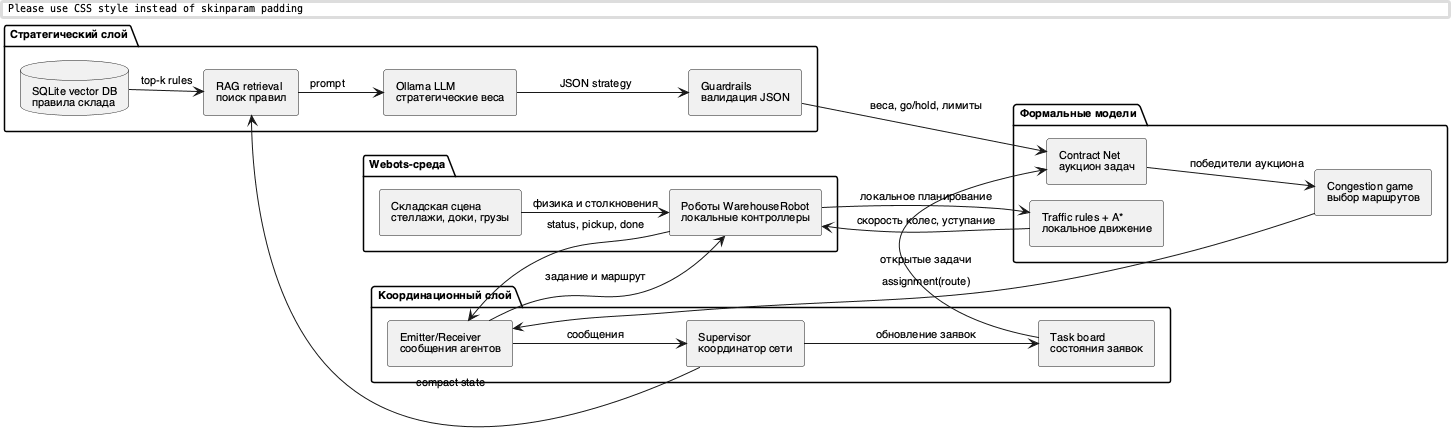
\includegraphics[width=0.98\textwidth]{figures/uml/article_architecture.png}
\caption{Компонентная архитектура разработанной многоагентной системы.}
\label{fig:architecture}
\end{figure}

На рис.~\ref{fig:architecture} показано соответствие программных компонентов уровням принятия решений. Контроллеры роботов формируют поток событий, supervisor поддерживает снимок состояния склада, RAG-модуль извлекает правила из локальной SQLite vector DB, LLM-слой возвращает стратегический JSON, а модуль формальных моделей выполняет Contract Net и игру с заторами. Такое разделение необходимо для воспроизводимости: если Ollama недоступна или возвращает некорректный JSON, используется детерминированная fallback-стратегия, а Contract Net и игра с заторами продолжают работать.

\begin{figure}[!htbp]
\centering
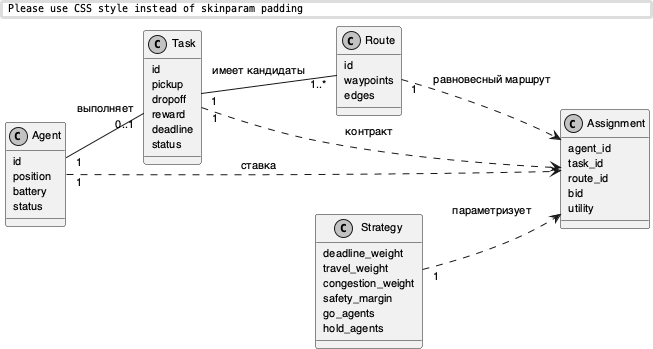
\includegraphics[width=0.78\textwidth]{figures/uml/article_model.png}
\caption{Упрощенная предметная UML-модель сущностей задачи.}
\label{fig:model}
\end{figure}

Предметная модель на рис.~\ref{fig:model} соответствует программным классам \texttt{AgentSnapshot}, \texttt{Task}, \texttt{Route}, \texttt{Strategy} и \texttt{Assignment}. Сущность \texttt{Strategy} является связующим элементом между LLM-слоем и формальными алгоритмами. Она содержит только численные и дискретные параметры, которые затем нормализуются и ограничиваются допустимыми диапазонами.

\begin{figure}[!htbp]
\centering
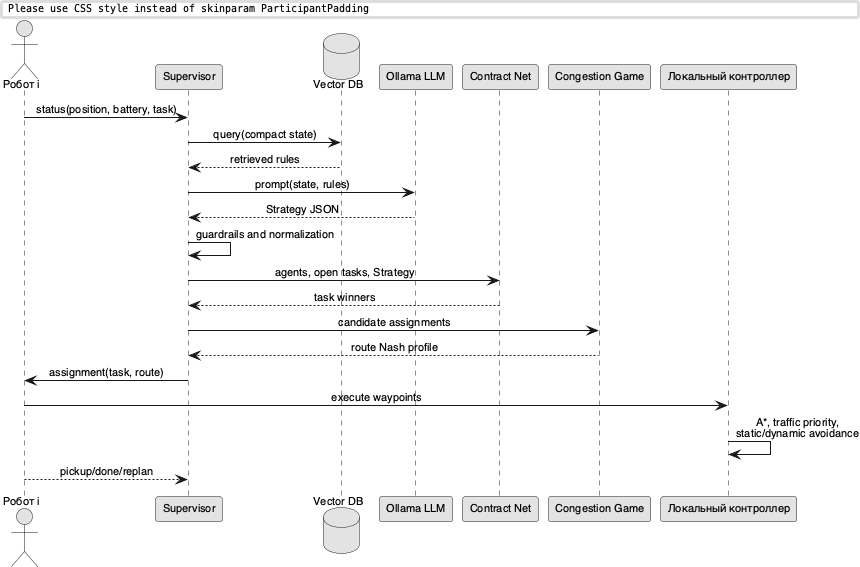
\includegraphics[width=0.82\textwidth]{figures/uml/article_decision_pipeline.png}
\caption{Последовательность принятия решений от состояния склада до локального исполнения маршрута.}
\label{fig:pipeline}
\end{figure}

Диаграмма последовательности на рис.~\ref{fig:pipeline} показывает один цикл принятия решений. Сначала роботы отправляют сообщения о состоянии. Затем supervisor формирует $z_t$ и вызывает стратегический уровень. Если активна LLM-стратегия, RAG извлекает правила, Ollama возвращает JSON, а guardrails строят стратегический вектор. После этого Contract Net назначает задачи агентам, congestion game выбирает маршруты с учетом текущих и стратегических штрафов, а сообщения назначения отправляются конкретным роботам.

Операционный уровень реализован в индивидуальных контроллерах роботов. Робот получает назначение, строит путь по waypoints, при необходимости перестраивает локальный объезд через A*, учитывает статические препятствия и safety disks других роботов, затем сообщает события \texttt{pickup}, \texttt{done} и \texttt{replan}. Таким образом, архитектура является гибридной: стратегический контекст задается LLM, но безопасность и движение определяются явными алгоритмами.

\section{Описание экспериментов}

Экспериментальная оценка проверяет не сам факт работы LLM, а системный эффект от ее включения в поток данных на рис.~\ref{fig:data-flow}. Проверяемая гипотеза состоит в следующем: LLM-слой должен ухудшать или не улучшать малые сцены, где достаточно fallback-правил, но может дать выигрыш в конфигурации, где текстовое правило о перегруженном центральном коридоре должно быть преобразовано в стратегические веса, ограничения допуска и перераспределение потока по обходным маршрутам.

Для проверки рассмотрены четыре сценария: большая базовая сцена с 3 задачами и 4 роботами (L-3), большая сцена с 9 задачами и 8 роботами (L-9), большая сцена обслуживания с 9 задачами и 8 роботами (LM-9), а также вычислительная сцена с 12 задачами и 10 роботами (H-12). Основная Webots-конфигурация соответствует сценарию LM-9, поскольку именно в ней центральный коридор не закрыт жестко, но получает высокий контекстный штраф из-за инспекционного трафика.

Сравнивались два режима. В режиме \textit{fallback} стратегия задавалась детерминированными правилами без обращения к LLM. В режиме \textit{llm} использовались SQLite vector DB, RAG, Ollama \texttt{qwen2.5:0.5b} и guardrails. В обоих режимах неизменными оставались Contract Net, congestion game, локальные правила движения и A*. Поэтому различие результатов связано не с заменой планировщика, а с изменением стратегического вектора. Метрики включали makespan, суммарное ожидание, суммарную дистанцию, число поздних задач, количество выбранных bypass-маршрутов и задержку LLM-запроса. Численные результаты получены в headless-эксперименте, использующем те же формальные модели назначения и маршрутизации, что и Webots-контроллеры; Webots-сцена дополнительно использовалась для проверки геометрии, сетевого взаимодействия контроллеров и визуальной воспроизводимости сценария.

Метрики вычислялись по журналу событий. Пусть $C_\tau$ -- момент завершения заявки $\tau$, $r_\tau$ -- выбранный маршрут, $L(r_\tau)$ -- его длина, $W_\tau$ -- суммарное время ожидания заявки до фактического начала движения назначенного робота. Тогда
\[
M=\max_{\tau \in T} C_\tau
\]
задает makespan, а
\[
W=\sum_{\tau \in T} W_\tau,\qquad
D=\sum_{\tau \in T} L(r_\tau)
\]
задают суммарное ожидание и суммарную дистанцию. Число bypass-маршрутов определяется как
\[
B=\sum_{\tau \in T}\mathbb{I}(r_\tau \in R_\tau^{bypass}),
\]
где $R_\tau^{bypass}$ -- множество маршрутов, проходящих по периферийным коридорам. Доля завершенных задач
\[
P=\frac{|\{\tau:C_\tau < \infty\}|}{|T|}
\]
использовалась как контроль работоспособности сценария. Для сравнения режимов применялись относительные изменения $\Delta M=(M_{fallback}-M_{llm})/M_{fallback}$ и $\Delta W=(W_{fallback}-W_{llm})/W_{fallback}$. Положительное значение этих величин означает выигрыш LLM-режима.

Важным элементом методики является сопоставимость режимов. В обоих случаях набор заявок, координаты роботов, граф склада и локальные правила движения совпадали. Отличались только значения $\Theta$: в fallback-режиме они вычислялись детерминированно, а в LLM-режиме извлекались из ответа Ollama после RAG и guardrails. Это исключает ситуацию, при которой выигрыш объясняется изменением низкоуровневого контроллера или геометрии сцены.

\begin{table}[!htbp]
\centering
\caption{Результаты вычислительного эксперимента LLM против fallback.}
\label{tab:experiment}
\scriptsize
\begin{tabular}{llrrrrrrrr}
\toprule
Сценарий & Режим & Роб. & Зад. & Вып. & Makespan & Wait & Dist. & Bypass & LLM, с \\
\midrule
L-3 & fallback & 4 & 3 & 3 & 138.0 & 4.5 & 169.8 & 0 & 0.000 \\
L-3 & llm & 4 & 3 & 3 & 157.5 & 0.0 & 194.4 & 2 & 8.589 \\
L-9 & fallback & 8 & 9 & 9 & 256.5 & 73.5 & 548.6 & 3 & 0.000 \\
L-9 & llm & 8 & 9 & 9 & 259.5 & 70.5 & 587.0 & 6 & 8.480 \\
LM-9 & fallback & 8 & 9 & 9 & 294.0 & 472.5 & 548.6 & 3 & 0.000 \\
LM-9 & llm & 8 & 9 & 9 & 252.0 & 28.5 & 587.0 & 6 & 9.809 \\
H-12 & fallback & 10 & 12 & 12 & 315.0 & 133.5 & 838.5 & 3 & 0.000 \\
H-12 & llm & 10 & 12 & 12 & 316.5 & 106.5 & 912.9 & 8 & 11.159 \\
\bottomrule
\end{tabular}
\end{table}

Наиболее выраженный выигрыш наблюдается в сценарии LM-9. Makespan снижается на 42.0 с, что соответствует относительному улучшению 14.3\%. Суммарное ожидание снижается на 444.0 с, или на 94.0\%. При этом суммарная дистанция возрастает с 548.6 до 587.0, поскольку LLM-стратегия чаще использует обходы. Задержка LLM-запроса в данном сценарии составила 9.809 с и окупилась только вследствие существенного снижения ожидания. Следовательно, эффект подхода состоит не в нахождении кратчайших маршрутов, а в более раннем переводе части потока с потенциально конфликтного центра на обходы и в дозированном выпуске роботов.

В малой сцене с 3 задачами LLM ухудшает makespan, поскольку выбирает более осторожную стратегию обходов при отсутствии существенного конфликта. В крупной вычислительной сцене с 12 задачами LLM снижает ожидание, но не улучшает makespan: дополнительные обходы увеличивают путь и компенсируют выигрыш от меньшего ожидания. Следовательно, целесообразность LLM зависит от структуры среды. Необходимы одновременно три условия: наличие альтернативных маршрутов, достаточное число конкурирующих заявок и контекстное правило, которое нельзя выразить простым постоянным fallback-весом.

\begin{figure}[!htbp]
\centering
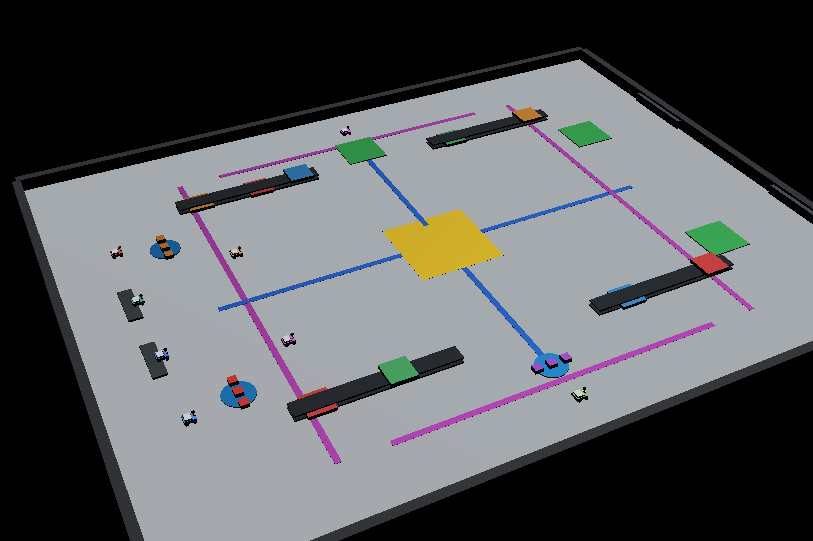
\includegraphics[width=0.78\textwidth]{figures/screenshots/webots_scene_0000.png}
\caption{Кадр Webots-сцены: склад, маршруты, грузы и восемь роботов в начальном состоянии.}
\label{fig:webots-scene}
\end{figure}

\begin{figure}[!htbp]
\centering
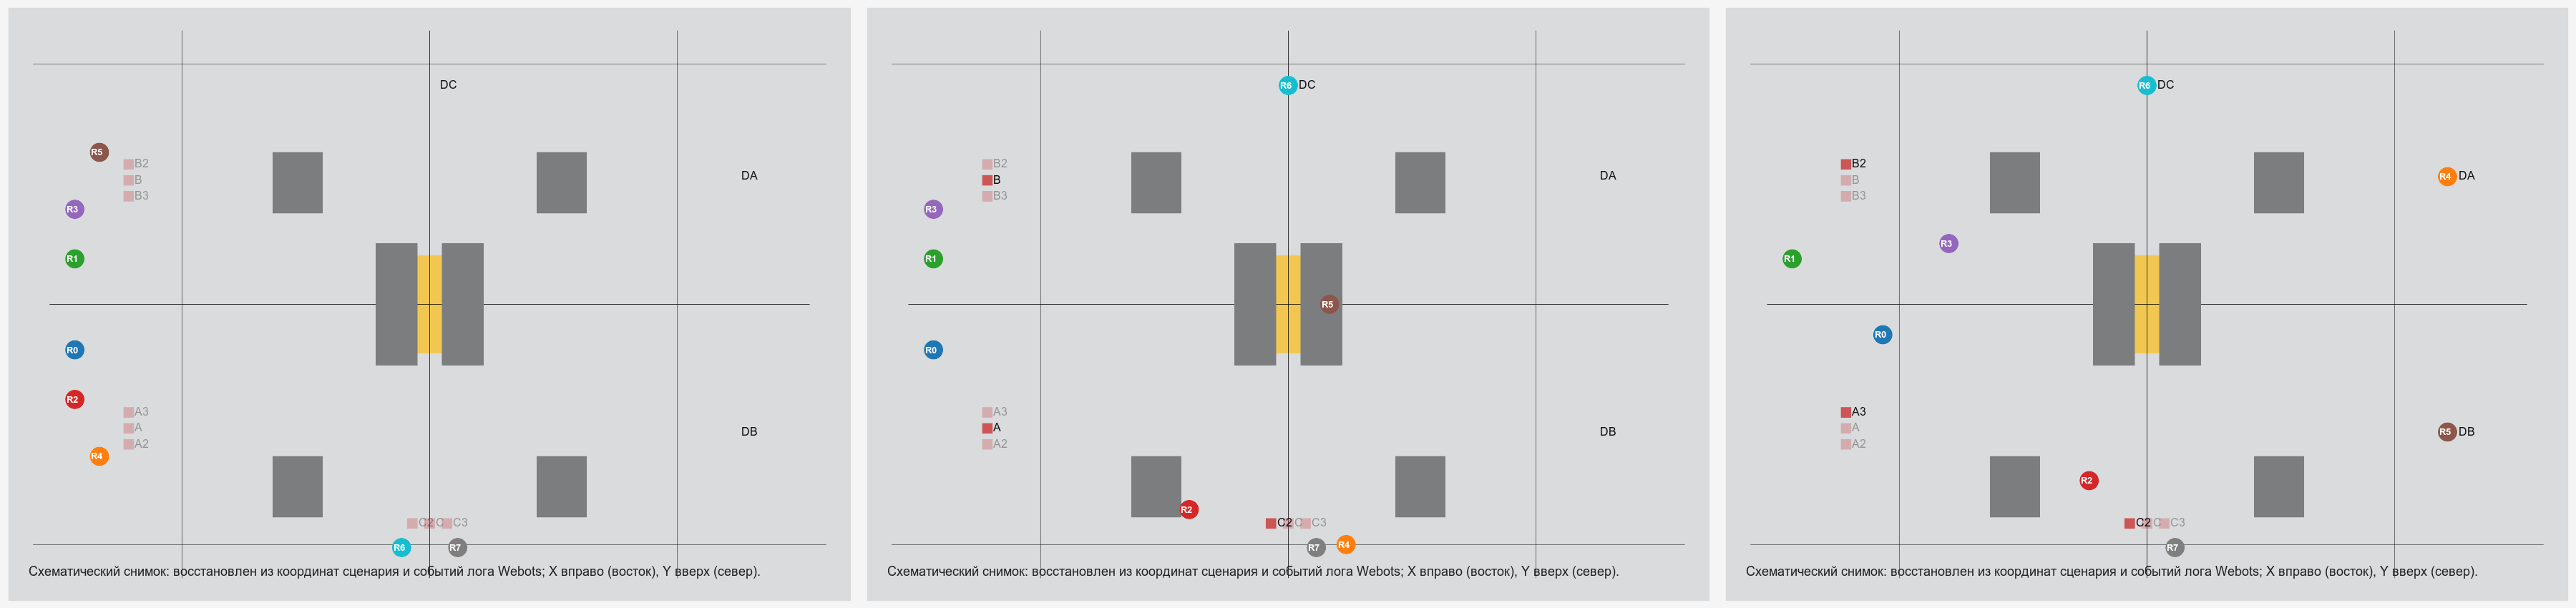
\includegraphics[width=0.94\textwidth]{figures/experiment_snapshots_montage.png}
\caption{Схематические снимки хода эксперимента, восстановленные из координат сценария и событий Webots-лога: начальное состояние, выполнение первых заявок и запуск повторных задач.}
\label{fig:snapshots}
\end{figure}

Рис.~\ref{fig:webots-scene} показывает структуру основной сцены Webots. Рис.~\ref{fig:snapshots} иллюстрирует динамику исполнения: сначала LLM/RAG разрешает выпуск трех роботов к семействам A/B/C, затем после завершения одной из доставок Contract Net назначает следующую задачу с учетом свободных зон. Повторные задачи не открываются искусственными волнами: все заявки доступны с начала, но допуск к исполнению регулируется стратегией и ограничениями семей зон.

\section{Обсуждение}

Полученные результаты подтверждают центральное предположение работы: роль LLM в многоагентной робототехнике должна быть ограничена стратегической параметризацией. LLM интерпретирует правила и состояние склада, но не принимает физически исполнимые решения. Физически значимые решения остаются в формальных моделях: Contract Net определяет соответствие агент--заявка, игра с заторами выбирает маршрутный профиль, а локальный контроллер обеспечивает движение и безопасность.

Системный эффект возникает благодаря изменению причинной цепочки принятия решений. В fallback-режиме центр остается привлекательным, пока локальные или тактические штрафы не становятся достаточно большими. В LLM-режиме текстовое правило об инспекционном трафике заранее повышает вес заторов и ограничивает одновременный выпуск роботов. Поэтому часть агентов выбирает более длинные обходы, но суммарное ожидание резко уменьшается. Такой результат объясняет, почему рост дистанции не является недостатком сам по себе: в конфликтной среде более длинный маршрут может уменьшать глобальное время завершения.

Вместе с тем подход имеет четкие границы применимости. Для малых сцен стоимость LLM-запроса и избыточная осторожность могут ухудшить результат. При отсутствии альтернативных маршрутов LLM не имеет механизма для полезного перераспределения потока. При слишком большом числе задач без дополнительных структурных ограничений LLM может снижать ожидание, но не обязательно уменьшать makespan. Наиболее целесообразной областью применения являются сценарии с 8 и более роботами, 9 и более открытыми заявками, конфликтным центральным коридором и несколькими обходными маршрутами.

Отдельно следует отметить вопрос доверия к LLM-ответу. В разработанной системе ответ модели не используется напрямую. Он проходит фильтрацию типов, ограничение численных диапазонов, проверку идентификаторов роботов и ребер, а также преобразуется в одноразовый диспетчерский шлюз. Такой подход снижает риск некорректного поведения и сохраняет работоспособность системы при отказе Ollama.

С точки зрения внутренней валидности основным ограничением эксперимента является использование одного детерминированного набора сценариев. Это оправдано для демонстрации механизма и причинной связи между правилами, стратегическим вектором и маршрутами, но недостаточно для утверждения о статистической устойчивости эффекта. Поэтому численные значения следует интерпретировать как результат вычислительного эксперимента на специально сконструированных конфигурациях, а не как универсальную оценку всех складских MAS.

С точки зрения внешней валидности важны два ограничения. Во-первых, Webots-сцена моделирует транспортную задачу на уровне мобильных платформ и waypoint-маршрутов; операции захвата, точного позиционирования под грузом и взаимодействия с реальными стеллажами представлены упрощенно. Во-вторых, локальная embedding-модель векторной базы намеренно проста, поскольку целью было показать архитектурную роль RAG, а не максимизировать качество семантического поиска. В промышленной системе эту часть следует заменить на специализированные эмбеддинги и расширенную онтологию складских правил.

Тем не менее указанные ограничения не отменяют ключевой результат: эффект LLM проявляется только тогда, когда она влияет на формальные параметры, имеющие причинную связь с конфликтами движения. Если retrieved rules не меняют веса заторов, лимиты выпуска или множества $A^{go}$ и $A^{hold}$, то LLM становится дорогостоящей текстовой надстройкой. Если же правила изменяют именно эти параметры, то система получает измеримый механизм перераспределения потока без передачи LLM прямого управления роботам.

\section{Выводы и направления дальнейших исследований}

В работе предложена и реализована многоуровневая система управления складской группой роботов, объединяющая RAG-LLM, Contract Net Protocol, игру с заторами и локальное предотвращение столкновений. Объектом исследования выступала складская многоагентная робототехническая система, а предметом -- механизм преобразования текстовых правил эксплуатации в параметры формальных моделей координации. Основной результат состоит в том, что LLM может быть полезна при строгом ограничении ее роли: она формирует стратегический вектор, но не управляет роботами напрямую.

Научная новизна состоит в RAG-LLM-параметризации формальных моделей назначения и маршрутизации, описанной через логико-алгебраическую модель и диаграмму потоков данных. Практический эффект показан в сценарии LM-9: makespan снижен на 14.3\%, а суммарное ожидание -- на 94.0\% при сохранении тех же тактических и операционных алгоритмов. Одновременно результаты показывают, что LLM не является универсальным улучшением: в малой сцене она ухудшает makespan, а в сверхкрупной сцене снижает ожидание без улучшения времени завершения.

Дальнейшие исследования целесообразно вести в четырех направлениях. Первое направление состоит в переходе от эвристического guardrail к формальной верификации LLM-стратегии. Второе направление связано с расширением векторной базы до онтологии складских правил и нормативных ограничений. Третье направление предполагает перенос модели на стандартные мобильные манипуляторы, включая KUKA youBot, с явным моделированием операций захвата и разгрузки. Четвертое направление состоит в проведении серии статистических экспериментов с несколькими случайными семенами, чтобы оценить устойчивость выигрыша LLM по доверительным интервалам.

\bibliographystyle{splncs04}
\bibliography{references}

\end{document}
